\section{Исследовательский раздел}

В данном разделе будет проведено исследование зависимости времени обработки URB от работы демона.

\subsection{Описание исследования}

Замер времени будет происходить для функции драйвера \texttt{jskbd\_complete} с использованием функции ядра \texttt{ktime\_get} \cite{ktime-get}, для двух сценариев:

\begin{itemize}[leftmargin=1.6\parindent]
    \item при запущенном демоне;
    \item при остановленном демоне.
\end{itemize}

При сравнении будут учитываться только первые 1000 измерений с момента запуска драйвера и подключения геймпада. В результате анализа полученных данных будут рассчитаны и сопоставлены средние значения измерений.

\subsection{Технические характеристики}

Исследование будет проводиться на ноутбуке Dell Vostro 14 5410. Характеристики системы приведены ниже.

\begin{itemize}[leftmargin=1.6\parindent]
    \item Процессор: 11th Gen Intel i7-11370H (8) @ 4.800GHz.
    \item Оперативная память: 8 ГБ.
    \item Операционная система: Arch Linux x86\_64.
    \item Графическая оболочка: KDE Plasma 5.26.4.
\end{itemize}

\subsection{Результаты исследования}

На рисунке \ref{fig:result} приведены результаты в виде гистограммы для всех полученных измерений.

\begin{figure}[ht]
    \centering
    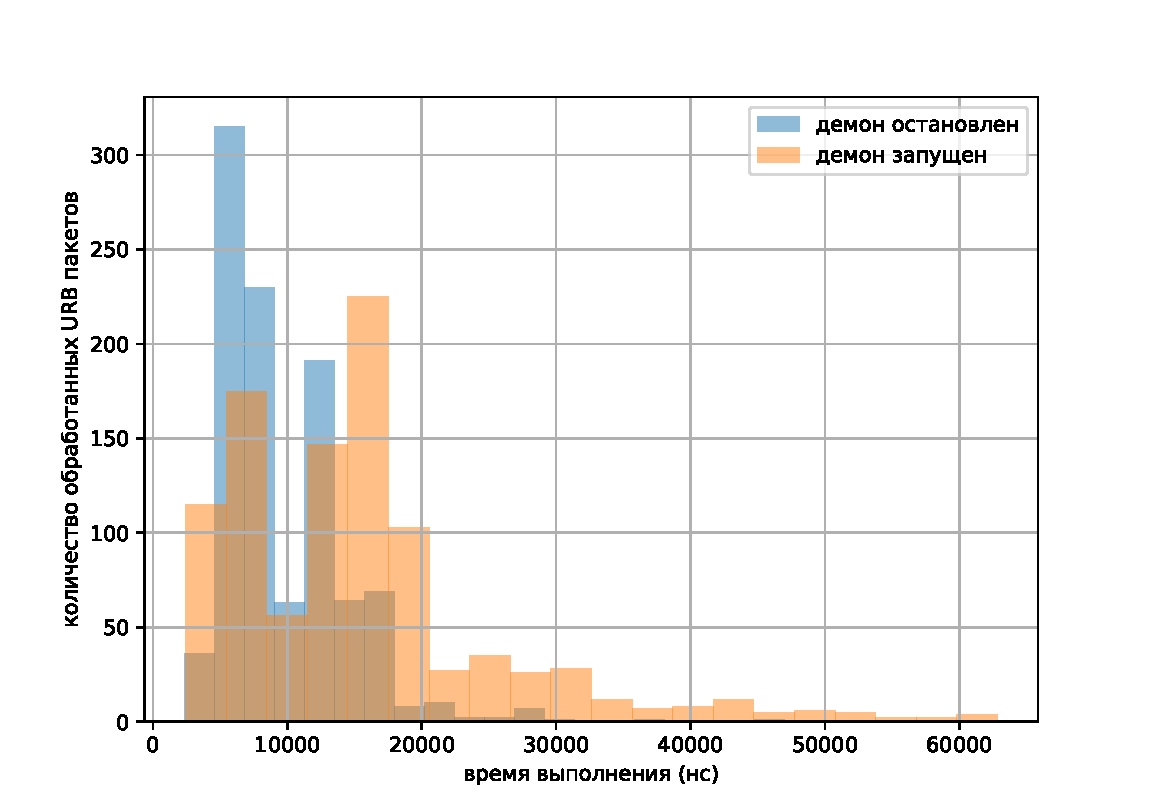
\includegraphics[width=\linewidth]{img/figure.pdf}
    \caption{Результаты замеров времени для двух сценариев}
    \label{fig:result}
\end{figure}

По результатам исследования установлены следующие средние значения обработки URB пакетов:

\begin{itemize}[leftmargin=1.6\parindent]
    \item при запущенном демоне: 15649 нс;
    \item при остановленном демоне: 9679 нс.
\end{itemize}

Данный результат можно объяснить тем, что запущенный демон требует больше времени на поддержание очереди ждущих процессов. Данное время в среднем можно считать равным 5970 нс.

\pagebreak
